% Generated by Sphinx.
\def\sphinxdocclass{report}
\documentclass[letterpaper,10pt,openany,oneside]{sphinxmanual}
\usepackage[utf8]{inputenc}
\DeclareUnicodeCharacter{00A0}{\nobreakspace}
\usepackage[T1]{fontenc}
\usepackage[english]{babel}
\usepackage{times}
\usepackage[Bjarne]{fncychap}
\usepackage{longtable}
\usepackage{sphinx}
\usepackage{multirow}


\title{Distributed Computing Fundamentals}
\date{July 26, 2013}
\release{}
\author{CSInParallel Project}
\newcommand{\sphinxlogo}{}
\renewcommand{\releasename}{}
\makeindex

\makeatletter
\def\PYG@reset{\let\PYG@it=\relax \let\PYG@bf=\relax%
    \let\PYG@ul=\relax \let\PYG@tc=\relax%
    \let\PYG@bc=\relax \let\PYG@ff=\relax}
\def\PYG@tok#1{\csname PYG@tok@#1\endcsname}
\def\PYG@toks#1+{\ifx\relax#1\empty\else%
    \PYG@tok{#1}\expandafter\PYG@toks\fi}
\def\PYG@do#1{\PYG@bc{\PYG@tc{\PYG@ul{%
    \PYG@it{\PYG@bf{\PYG@ff{#1}}}}}}}
\def\PYG#1#2{\PYG@reset\PYG@toks#1+\relax+\PYG@do{#2}}

\expandafter\def\csname PYG@tok@gd\endcsname{\def\PYG@tc##1{\textcolor[rgb]{0.63,0.00,0.00}{##1}}}
\expandafter\def\csname PYG@tok@gu\endcsname{\let\PYG@bf=\textbf\def\PYG@tc##1{\textcolor[rgb]{0.50,0.00,0.50}{##1}}}
\expandafter\def\csname PYG@tok@gt\endcsname{\def\PYG@tc##1{\textcolor[rgb]{0.00,0.25,0.82}{##1}}}
\expandafter\def\csname PYG@tok@gs\endcsname{\let\PYG@bf=\textbf}
\expandafter\def\csname PYG@tok@gr\endcsname{\def\PYG@tc##1{\textcolor[rgb]{1.00,0.00,0.00}{##1}}}
\expandafter\def\csname PYG@tok@cm\endcsname{\let\PYG@it=\textit\def\PYG@tc##1{\textcolor[rgb]{0.25,0.50,0.56}{##1}}}
\expandafter\def\csname PYG@tok@vg\endcsname{\def\PYG@tc##1{\textcolor[rgb]{0.73,0.38,0.84}{##1}}}
\expandafter\def\csname PYG@tok@m\endcsname{\def\PYG@tc##1{\textcolor[rgb]{0.13,0.50,0.31}{##1}}}
\expandafter\def\csname PYG@tok@mh\endcsname{\def\PYG@tc##1{\textcolor[rgb]{0.13,0.50,0.31}{##1}}}
\expandafter\def\csname PYG@tok@cs\endcsname{\def\PYG@tc##1{\textcolor[rgb]{0.25,0.50,0.56}{##1}}\def\PYG@bc##1{\setlength{\fboxsep}{0pt}\colorbox[rgb]{1.00,0.94,0.94}{\strut ##1}}}
\expandafter\def\csname PYG@tok@ge\endcsname{\let\PYG@it=\textit}
\expandafter\def\csname PYG@tok@vc\endcsname{\def\PYG@tc##1{\textcolor[rgb]{0.73,0.38,0.84}{##1}}}
\expandafter\def\csname PYG@tok@il\endcsname{\def\PYG@tc##1{\textcolor[rgb]{0.13,0.50,0.31}{##1}}}
\expandafter\def\csname PYG@tok@go\endcsname{\def\PYG@tc##1{\textcolor[rgb]{0.19,0.19,0.19}{##1}}}
\expandafter\def\csname PYG@tok@cp\endcsname{\def\PYG@tc##1{\textcolor[rgb]{0.00,0.44,0.13}{##1}}}
\expandafter\def\csname PYG@tok@gi\endcsname{\def\PYG@tc##1{\textcolor[rgb]{0.00,0.63,0.00}{##1}}}
\expandafter\def\csname PYG@tok@gh\endcsname{\let\PYG@bf=\textbf\def\PYG@tc##1{\textcolor[rgb]{0.00,0.00,0.50}{##1}}}
\expandafter\def\csname PYG@tok@ni\endcsname{\let\PYG@bf=\textbf\def\PYG@tc##1{\textcolor[rgb]{0.84,0.33,0.22}{##1}}}
\expandafter\def\csname PYG@tok@nl\endcsname{\let\PYG@bf=\textbf\def\PYG@tc##1{\textcolor[rgb]{0.00,0.13,0.44}{##1}}}
\expandafter\def\csname PYG@tok@nn\endcsname{\let\PYG@bf=\textbf\def\PYG@tc##1{\textcolor[rgb]{0.05,0.52,0.71}{##1}}}
\expandafter\def\csname PYG@tok@no\endcsname{\def\PYG@tc##1{\textcolor[rgb]{0.38,0.68,0.84}{##1}}}
\expandafter\def\csname PYG@tok@na\endcsname{\def\PYG@tc##1{\textcolor[rgb]{0.25,0.44,0.63}{##1}}}
\expandafter\def\csname PYG@tok@nb\endcsname{\def\PYG@tc##1{\textcolor[rgb]{0.00,0.44,0.13}{##1}}}
\expandafter\def\csname PYG@tok@nc\endcsname{\let\PYG@bf=\textbf\def\PYG@tc##1{\textcolor[rgb]{0.05,0.52,0.71}{##1}}}
\expandafter\def\csname PYG@tok@nd\endcsname{\let\PYG@bf=\textbf\def\PYG@tc##1{\textcolor[rgb]{0.33,0.33,0.33}{##1}}}
\expandafter\def\csname PYG@tok@ne\endcsname{\def\PYG@tc##1{\textcolor[rgb]{0.00,0.44,0.13}{##1}}}
\expandafter\def\csname PYG@tok@nf\endcsname{\def\PYG@tc##1{\textcolor[rgb]{0.02,0.16,0.49}{##1}}}
\expandafter\def\csname PYG@tok@si\endcsname{\let\PYG@it=\textit\def\PYG@tc##1{\textcolor[rgb]{0.44,0.63,0.82}{##1}}}
\expandafter\def\csname PYG@tok@s2\endcsname{\def\PYG@tc##1{\textcolor[rgb]{0.25,0.44,0.63}{##1}}}
\expandafter\def\csname PYG@tok@vi\endcsname{\def\PYG@tc##1{\textcolor[rgb]{0.73,0.38,0.84}{##1}}}
\expandafter\def\csname PYG@tok@nt\endcsname{\let\PYG@bf=\textbf\def\PYG@tc##1{\textcolor[rgb]{0.02,0.16,0.45}{##1}}}
\expandafter\def\csname PYG@tok@nv\endcsname{\def\PYG@tc##1{\textcolor[rgb]{0.73,0.38,0.84}{##1}}}
\expandafter\def\csname PYG@tok@s1\endcsname{\def\PYG@tc##1{\textcolor[rgb]{0.25,0.44,0.63}{##1}}}
\expandafter\def\csname PYG@tok@gp\endcsname{\let\PYG@bf=\textbf\def\PYG@tc##1{\textcolor[rgb]{0.78,0.36,0.04}{##1}}}
\expandafter\def\csname PYG@tok@sh\endcsname{\def\PYG@tc##1{\textcolor[rgb]{0.25,0.44,0.63}{##1}}}
\expandafter\def\csname PYG@tok@ow\endcsname{\let\PYG@bf=\textbf\def\PYG@tc##1{\textcolor[rgb]{0.00,0.44,0.13}{##1}}}
\expandafter\def\csname PYG@tok@sx\endcsname{\def\PYG@tc##1{\textcolor[rgb]{0.78,0.36,0.04}{##1}}}
\expandafter\def\csname PYG@tok@bp\endcsname{\def\PYG@tc##1{\textcolor[rgb]{0.00,0.44,0.13}{##1}}}
\expandafter\def\csname PYG@tok@c1\endcsname{\let\PYG@it=\textit\def\PYG@tc##1{\textcolor[rgb]{0.25,0.50,0.56}{##1}}}
\expandafter\def\csname PYG@tok@kc\endcsname{\let\PYG@bf=\textbf\def\PYG@tc##1{\textcolor[rgb]{0.00,0.44,0.13}{##1}}}
\expandafter\def\csname PYG@tok@c\endcsname{\let\PYG@it=\textit\def\PYG@tc##1{\textcolor[rgb]{0.25,0.50,0.56}{##1}}}
\expandafter\def\csname PYG@tok@mf\endcsname{\def\PYG@tc##1{\textcolor[rgb]{0.13,0.50,0.31}{##1}}}
\expandafter\def\csname PYG@tok@err\endcsname{\def\PYG@bc##1{\setlength{\fboxsep}{0pt}\fcolorbox[rgb]{1.00,0.00,0.00}{1,1,1}{\strut ##1}}}
\expandafter\def\csname PYG@tok@kd\endcsname{\let\PYG@bf=\textbf\def\PYG@tc##1{\textcolor[rgb]{0.00,0.44,0.13}{##1}}}
\expandafter\def\csname PYG@tok@ss\endcsname{\def\PYG@tc##1{\textcolor[rgb]{0.32,0.47,0.09}{##1}}}
\expandafter\def\csname PYG@tok@sr\endcsname{\def\PYG@tc##1{\textcolor[rgb]{0.14,0.33,0.53}{##1}}}
\expandafter\def\csname PYG@tok@mo\endcsname{\def\PYG@tc##1{\textcolor[rgb]{0.13,0.50,0.31}{##1}}}
\expandafter\def\csname PYG@tok@mi\endcsname{\def\PYG@tc##1{\textcolor[rgb]{0.13,0.50,0.31}{##1}}}
\expandafter\def\csname PYG@tok@kn\endcsname{\let\PYG@bf=\textbf\def\PYG@tc##1{\textcolor[rgb]{0.00,0.44,0.13}{##1}}}
\expandafter\def\csname PYG@tok@o\endcsname{\def\PYG@tc##1{\textcolor[rgb]{0.40,0.40,0.40}{##1}}}
\expandafter\def\csname PYG@tok@kr\endcsname{\let\PYG@bf=\textbf\def\PYG@tc##1{\textcolor[rgb]{0.00,0.44,0.13}{##1}}}
\expandafter\def\csname PYG@tok@s\endcsname{\def\PYG@tc##1{\textcolor[rgb]{0.25,0.44,0.63}{##1}}}
\expandafter\def\csname PYG@tok@kp\endcsname{\def\PYG@tc##1{\textcolor[rgb]{0.00,0.44,0.13}{##1}}}
\expandafter\def\csname PYG@tok@w\endcsname{\def\PYG@tc##1{\textcolor[rgb]{0.73,0.73,0.73}{##1}}}
\expandafter\def\csname PYG@tok@kt\endcsname{\def\PYG@tc##1{\textcolor[rgb]{0.56,0.13,0.00}{##1}}}
\expandafter\def\csname PYG@tok@sc\endcsname{\def\PYG@tc##1{\textcolor[rgb]{0.25,0.44,0.63}{##1}}}
\expandafter\def\csname PYG@tok@sb\endcsname{\def\PYG@tc##1{\textcolor[rgb]{0.25,0.44,0.63}{##1}}}
\expandafter\def\csname PYG@tok@k\endcsname{\let\PYG@bf=\textbf\def\PYG@tc##1{\textcolor[rgb]{0.00,0.44,0.13}{##1}}}
\expandafter\def\csname PYG@tok@se\endcsname{\let\PYG@bf=\textbf\def\PYG@tc##1{\textcolor[rgb]{0.25,0.44,0.63}{##1}}}
\expandafter\def\csname PYG@tok@sd\endcsname{\let\PYG@it=\textit\def\PYG@tc##1{\textcolor[rgb]{0.25,0.44,0.63}{##1}}}

\def\PYGZbs{\char`\\}
\def\PYGZus{\char`\_}
\def\PYGZob{\char`\{}
\def\PYGZcb{\char`\}}
\def\PYGZca{\char`\^}
\def\PYGZam{\char`\&}
\def\PYGZlt{\char`\<}
\def\PYGZgt{\char`\>}
\def\PYGZsh{\char`\#}
\def\PYGZpc{\char`\%}
\def\PYGZdl{\char`\$}
\def\PYGZti{\char`\~}
% for compatibility with earlier versions
\def\PYGZat{@}
\def\PYGZlb{[}
\def\PYGZrb{]}
\makeatother

\begin{document}

\maketitle
\tableofcontents
\phantomsection\label{index::doc}



\chapter{Instructor/Student Notes}
\label{Prerequisites/Prerequisites:distributed-computing-fundamentals}\label{Prerequisites/Prerequisites:instructor-student-notes}\label{Prerequisites/Prerequisites::doc}
Before getting started with this module, please keep in mind that we assume you have \textbf{some grasp of C programming}.

In the section called `Local Cluster Configuration' we provide some information about two types of clusters that are available at Macalester College.  If you are using this course module at your own institution, you will need to change this information to refer to your own cluster.

This module contains both background information and several activities for students to try using Message Passing Interface (MPI) programs on a cluster
of machines.  The examples and activities follow from simple introductory examples to activities, each of which increases in difficulty as you proceed.

\textbf{For the four activities, we recommend having the example code open in one window while you go through the explanation of the code.}  You can download them all here first, or there will be ways to dowload or look at each one in your browser as you go along.


\section{Files to try on your cluster}
\label{Prerequisites/Prerequisites:files-to-try-on-your-cluster}
The following examples are used in the next few pages of this module.  You can download each one (right-click and save) and eventually use a client such as scp to copy them up to a cluster machine.  \emph{However, they may already be available on your cluster. Check with your instructor.}

The first one is a complete zip file of all of them. The rest are each individual file.

Zip File:
\code{download dist\_example\_code.zip}

Simplest Hello World Example:
\code{download hellompi.c}

Hello World by Sending messages:
\code{download example2.c}

\textbf{Activity 1, Computing pi as area under the curve:}

\code{download mpi\_pi\_todo.c}

\code{download mpi\_pi\_done.c}

\textbf{Activity 2, Vector-Matrix Multiplication:}

\code{download vector\_matrix\_buggy\_todo.c}

\code{download vector\_matrix\_buggy\_done.c}

\textbf{Activity 3, Improved Vector-Matrix Multiplication}

\code{download vector\_matrix\_mpi\_todo.c}

\code{download vector\_matrix\_mpi.c}

\textbf{Activity 4, Matrix-Matrix Multiplication}

\code{download matrix\_multiplication\_todo.c}

\code{download matrix\_multiplication.c}


\chapter{Introduction to Cluster Computing}
\label{IntroCluster/IntroCluster:introduction-to-cluster-computing}\label{IntroCluster/IntroCluster::doc}
This course module is focused on distributed memory computing using a cluster of computers.
This sextion is a brief overview of parallel systems and clusters, designed to get you in the frame of mind for the examples you will try on a cluster.


\section{First, two parallel programming models}
\label{IntroCluster/IntroCluster:first-two-parallel-programming-models}
To prepare for what you will be working on, you need a basic understanding of parallel computer architectures. In particular, it is useful to know the difference between these two parallel computer architectures:
\begin{itemize}
\item {} 
Shared Memory Model

\item {} 
Distributed Memory Model

\end{itemize}

General Characteristics of Shared Memory Model:
\begin{description}
\item[{``}] \leavevmode\begin{itemize}
\item {} 
Shared memory parallel computers vary widely, but generally have in common the ability for all processors to access all memory as global address space.

\item {} 
Multiple processors can operate independently but share the same memory resources.

\item {} 
Changes in a memory location effected by one processor are visible to all other processors.'' {[}2{]}

\end{itemize}

\end{description}

{\hfill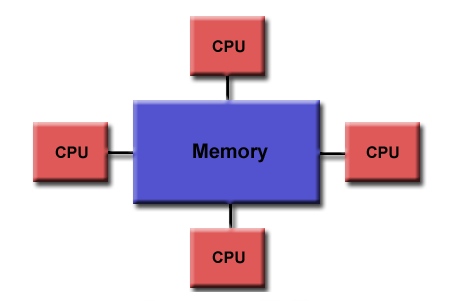
\includegraphics{SharedMemoryUMA.png}\hfill}

\begin{center}Figure 1: Shared Memory: Uniform Memory Access Obtained from www.computing.llnl.gov {[}3{]}
\end{center}
The rest of this course module is primarily focused on the distributed memory model of computing, which is different from the shared memory model.

According to {[}4{]}, the general characteristics of Distributed Memory Model are:
\begin{description}
\item[{\textbf{``}}] \leavevmode\begin{itemize}
\item {} 
Distributed memory systems require a communication network to connect inter-processor memory.

\item {} 
Processors have their own local memory. Memory addresses in one processor do not map to another processor, so there is no concept of global address space across all processors.

\item {} 
Because each processor has its own local memory, it operates independently. Changes it makes to its local memory have no effect on the memory of other processors. Hence, the concept of cache coherency does not apply.

\item {} 
When a processor needs access to data in another processor, it is usually the task of the programmer to explicitly define how and when data is communicated. Synchronization between tasks is likewise the programmer's responsibility.

\end{itemize}

\end{description}

\textbf{``}

{\hfill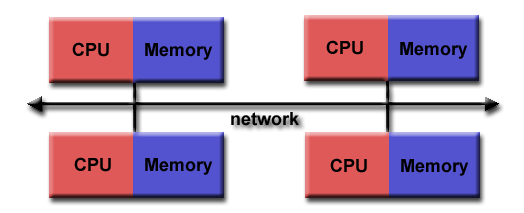
\includegraphics{DistributedMemory.png}\hfill}

\begin{center}Figure 2: Distributed Memory System Obtained from www.computing.llnl.gov {[}5{]}
\end{center}

\section{Clusters of Computers}
\label{IntroCluster/IntroCluster:clusters-of-computers}
Distributed Memory systems often manifest themseleves in the form of clusters of computers networked together over a high-speed network. Clusters of workstations connected through a highspeed switch are often called beowulf clusters.

\textbf{Definition}: A cluster is a type of parallel or distributed processing system, which consists of a collection of interconnected stand-alone computers cooperatively working together as a single, integrated computing resource. {[}1{]}

A cluster is usually a linux-based operating system. Basically, a cluster has four major components:
\begin{itemize}
\item {} 
Network is to provide communications between nodes and server.

\item {} 
Each node has its own processor, memory, and storage.

\item {} 
Server is to provide network services to the cluster.

\item {} 
Gateway acts as a firewall between the outside world and the cluster.

\end{itemize}

Some benefits of using clusters are:
\begin{itemize}
\item {} 
Inexpensive: Hardware and software of a cluster cost significantly much less than those of a supercomputer.

\item {} 
Scalability: extra nodes can be added to a cluster when work exceeds the capacities of the current system in the cluster.

\item {} 
Maintenance: A cluster is relatively easy to set up and maintain.

\item {} 
High Performance: Operations should be optimized and efficient.

\item {} 
Great capacity: Ability to solve a larger problem size.

\end{itemize}

There are many applications of clustering such as:
\begin{itemize}
\item {} 
Scientific computation

\item {} 
Parametric Simulations

\item {} 
Database Applications

\item {} 
Internet Applications

\item {} 
E-commerce Applications

\end{itemize}
\setbox0\vbox{
\begin{minipage}{0.95\linewidth}
\textbf{Recommended Reading:}

\medskip

\begin{itemize}
\item {} 
Please read \href{http://www.cloudbus.org/papers/ic\_cluster.pdf}{Cluster Computing: High-Performance, High-Availability, and High-Throughput Processing on a Network of Computers} {[}6{]}.

\item {} 
Case Studies on Cluster Applications: read from page 16 - 22.

\end{itemize}
\end{minipage}}
\begin{center}\setlength{\fboxsep}{5pt}\shadowbox{\box0}\end{center}

In order to use a cluster effectively, we need to have some programming environments such as Message Passing Interface (MPI), and OpenMP, etc. In this module, we will be learning about MPI on distributed memory cluster.
\paragraph{References}


\chapter{Local Cluster Configurations}
\label{LocalClusterConfig/LocalClusterConfig:local-cluster-configurations}\label{LocalClusterConfig/LocalClusterConfig::doc}
There are two local clusters at Macalester College, one is Selkie, and the other is LittleFe. Here we want to give you a sense of how the two clusters work.


\section{LittleFe}
\label{LocalClusterConfig/LocalClusterConfig:littlefe}
LittleFe is a 6-node distributed memory cluster. Each node is a motherboard consists of a CPU, I/O devices, and memory .etc. It uses Message Passing Interface (MPI) library to distribute the task to each node, and let each node work their own task simultaneously. Then we can combine the result from each node to get the overall output. Each node of LittleFe has nVidia GT 218 GPU, which enables LittleFe to do GPU programming, CUDA C. All the nodes connect via the network router.

LittleFe is Linux-based operating system, which is provided by Bootable Cluster CD (BCCD). BCCD also provides some cool applications that can be run using MPI such as GalaxSee, Life, and Parameter-space, etc. Because of LittleFe's ability, we have also been working on Heterogeneous programming model, which combines both CUDA and MPI. You will see in the next module. In this module, we will be using LittleFe for our MPI programming activities. Below is a picture of LittleFe.

{\hfill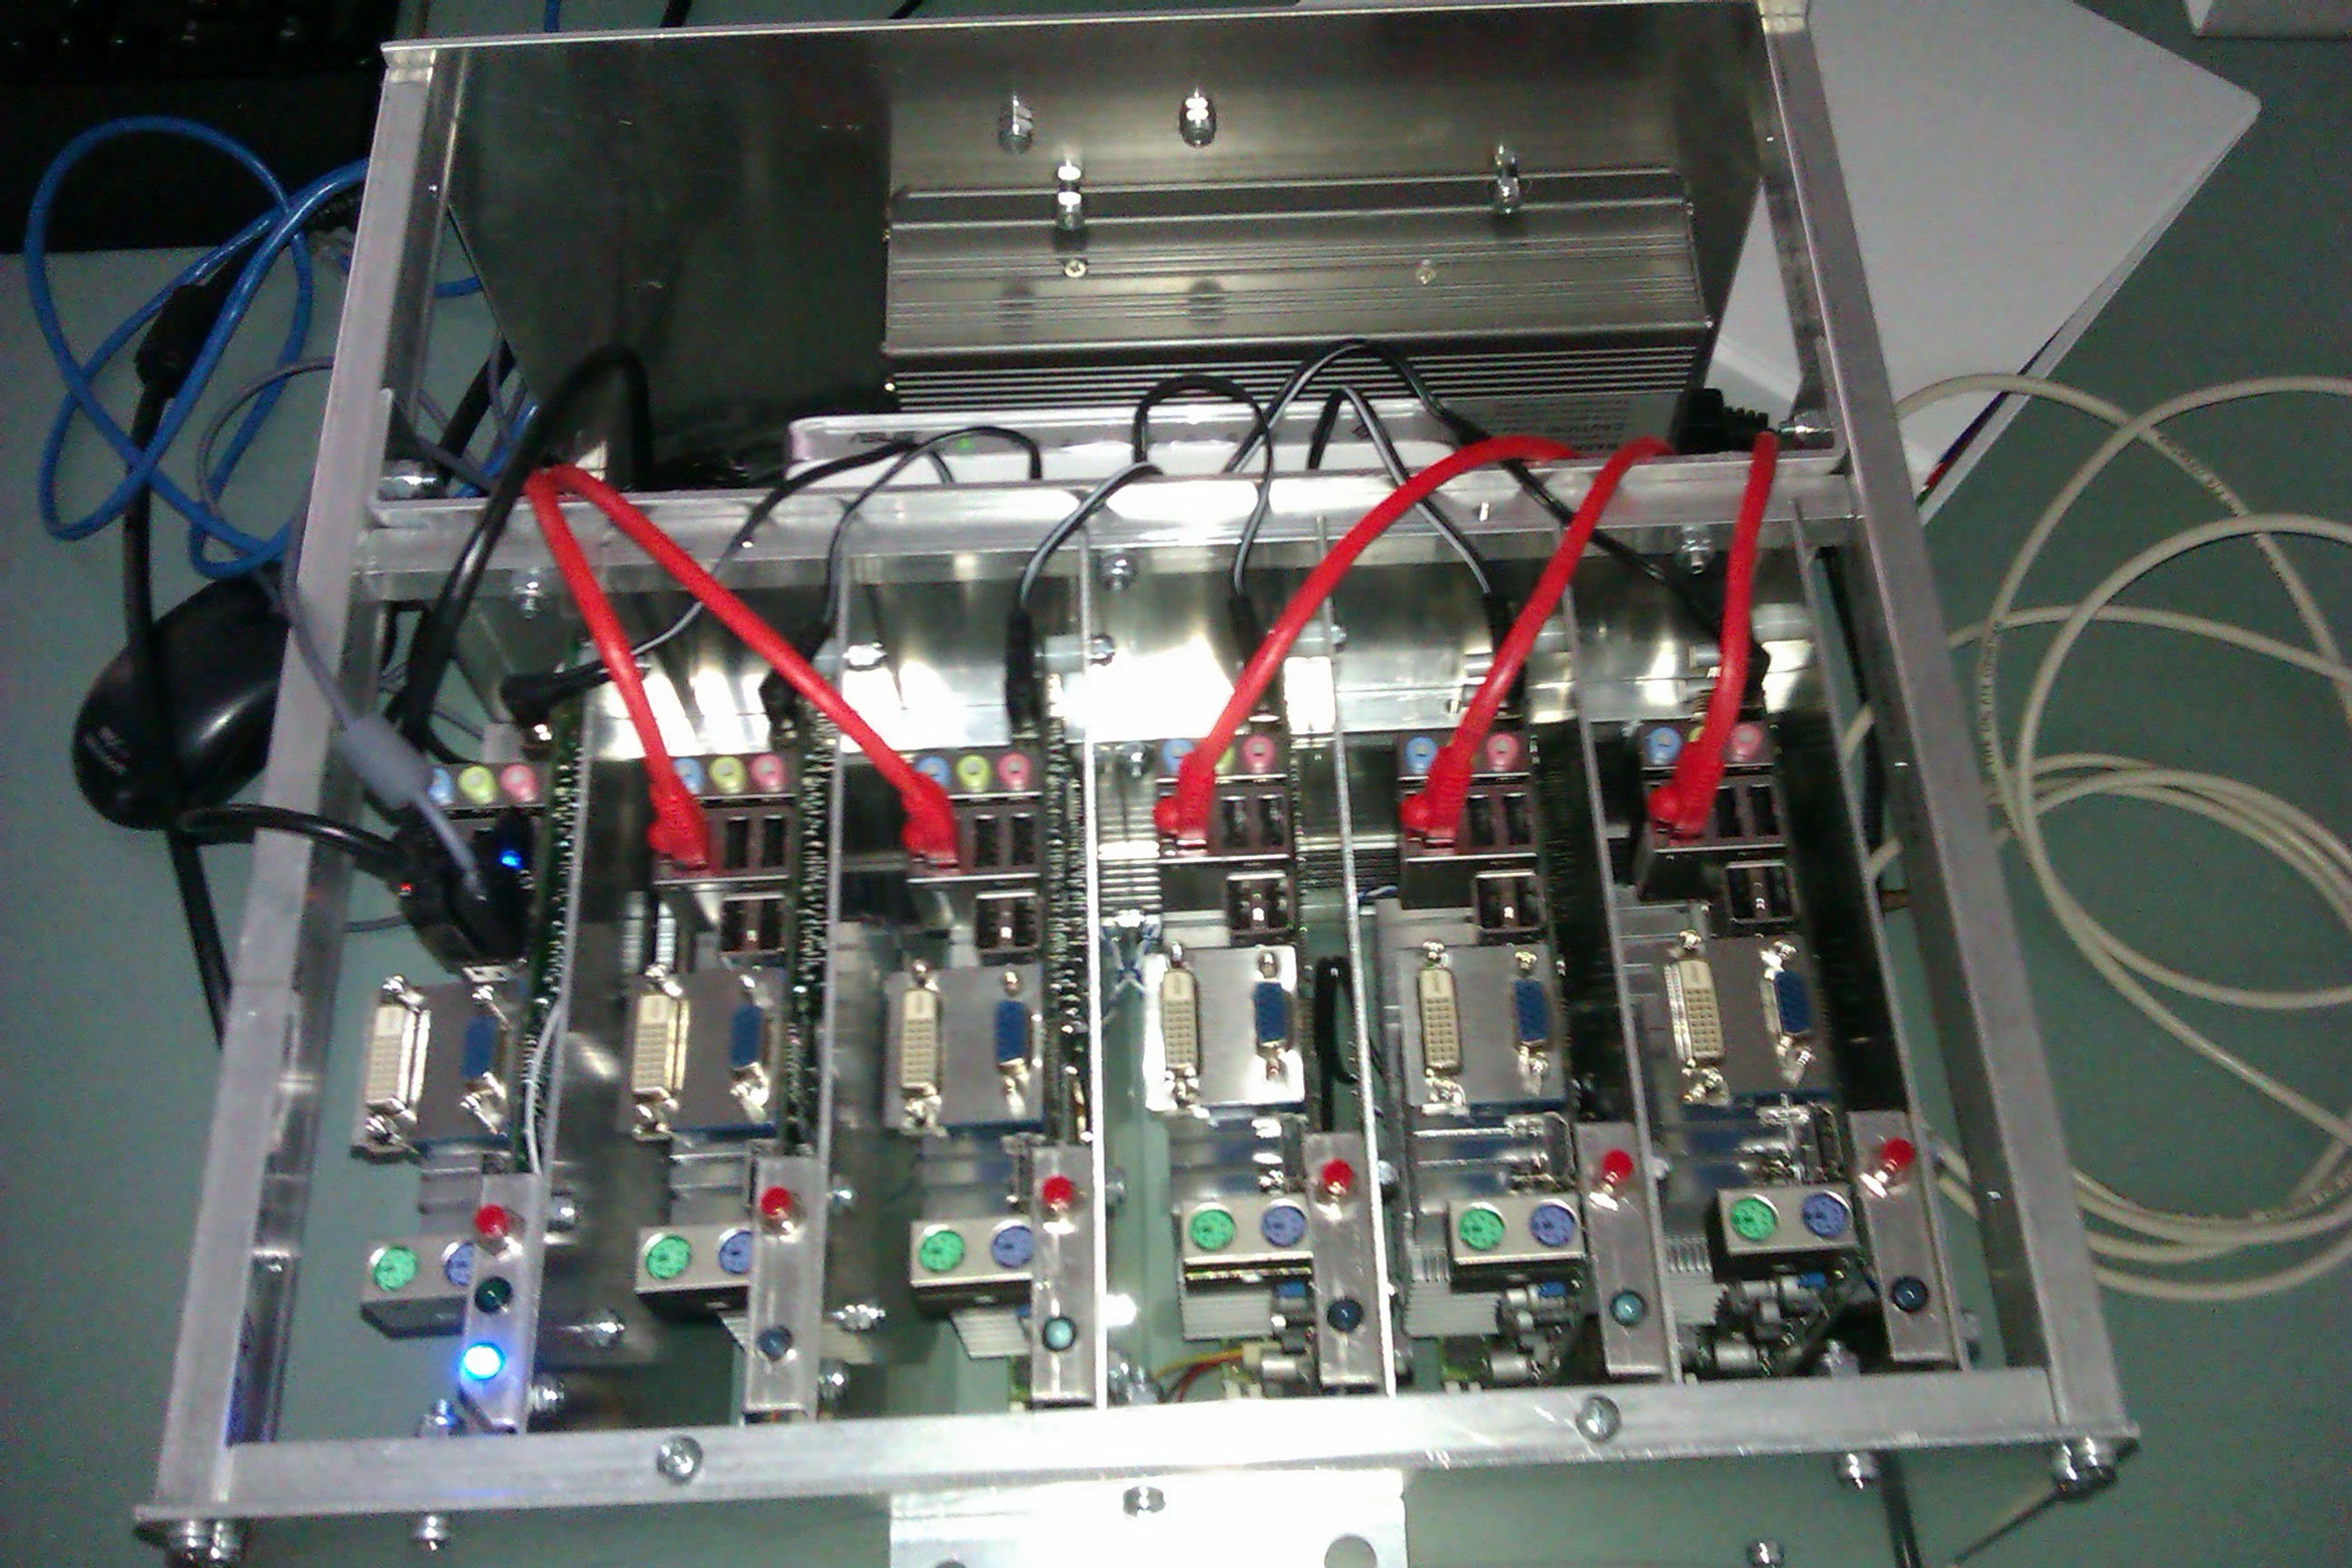
\includegraphics{LittleFe.jpg}\hfill}

\begin{center}Figure 1: LittleFe
\end{center}

\section{Selkie}
\label{LocalClusterConfig/LocalClusterConfig:selkie}
Selkie is a virtual cluster, which was built in summer 2011, at Macalester College by a computer science summer research group. Selkie currently consists of VMs running on 44 iMacs in the computer lab. Those iMacs machines are quad-core models, with 8 GB of RAM. Since these iMacs are used for other purposes as well, virtual machines have been set up as the guest operating system that is run inside a host operating system.  We used VirtualBox for virtual machines because VirtualBox runs on Mac OS X, and it is open source. The operating system configuration on each virtual machine is Ubuntu linix Server version 10.04. Each virtual machine uses 2 CPU cores and 4 GB of memory.
\setbox0\vbox{
\begin{minipage}{0.95\linewidth}
\textbf{Recommended Reading:}

\medskip

\begin{itemize}
\item {} 
To read more on \href{http://delivery.acm.org/10.1145/2160000/2157287/p517-shoop.pdf?ip=141.140.157.214\&acc=ACTIVE\%20SERVICE\&CFID=96092423\&CFTOKEN=89662159\&\_\_acm\_\_=1342713644\_7bcc228288bf005238f39f12e3a781c7}{Selkie Cluster}

\end{itemize}
\end{minipage}}
\begin{center}\setlength{\fboxsep}{5pt}\shadowbox{\box0}\end{center}


\subsection{How to log in onto your local clusters}
\label{LocalClusterConfig/LocalClusterConfig:how-to-log-in-onto-your-local-clusters}
Your instructor will provide the instructions of how to log in onto your local clusters.


\chapter{Introduction to MPI}
\label{introMPI/introMPI::doc}\label{introMPI/introMPI:introduction-to-mpi}

\section{What is MPI ?}
\label{introMPI/introMPI:what-is-mpi}
Message Passing Interface (MPI) is a subroutine or a library for passing messages between processes in a distributed memory model. MPI is not a programming language. MPI is a programming model that is widely used for parallel programming in a cluster. In the cluster, the head node is known as the master, and the other nodes are known as the workers. By using MPI, programmers are able to divide up the task and distribute each task to each worker or to some specific workers. Thus, each node can work on its own task simultaneously.

Since this is a small module, we will be focusing on only important and common MPI functions and techniques. For further study, there are a lot of free resources available on the Internet.


\section{Why MPI ?}
\label{introMPI/introMPI:why-mpi}
There are many reasons for using MPI as our parallel programming model:
\begin{itemize}
\item {} 
MPI is a standard message passing library, and it is supported on all high-performance computer platforms.

\item {} 
An MPI program is able to run on different platforms that support the MPI standard without changing your source codes.

\item {} 
Because of its parallel features, programmers are able to work on a much larger problem size with the faster computation.

\item {} 
There are many useful functions available in the MPI Library.

\item {} 
A variety of implementations are available.

\end{itemize}


\section{How do I write MPI program ?}
\label{introMPI/introMPI:how-do-i-write-mpi-program}
In order to get the MPI library working, you need to include the header file \textbf{\#include \textless{}mpi.h\textgreater{}} or \textbf{\#include “mpi.h”} in your C code.


\subsection{MPI Program Structure}
\label{introMPI/introMPI:mpi-program-structure}
Like other programming languages you have seen, program that includes MPI library has its structure. The structure is shown in the figure below:

{\hfill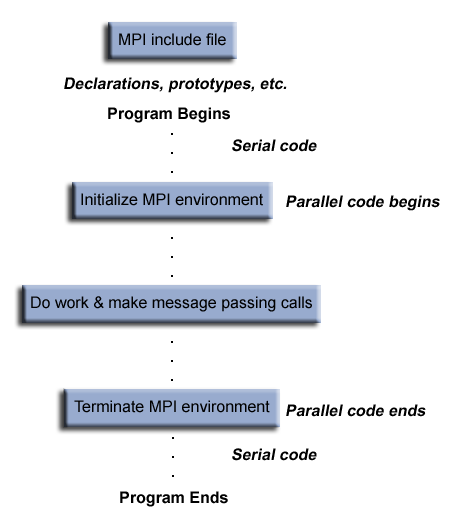
\includegraphics{MPIstructure.png}\hfill}

\begin{center}Figure 3: MPI program structure Obtained from computing.llnl.gov {[}1{]}
\end{center}
A MPI program is basically a C program that uses the MPI library, SO DON’T BE SCARED. The program has two different parts, one is serial, and the other is parallel. The serial part contains variable declarations, etc., and the parallel part starts when MPI execution environment has been initialized, and ends when MPI\_Finalize() has been called.

\textbf{Communicator}: a set of processes that have a valid rank of source or destination fields. The predefined communicator is MPI\_COMM\_WORLD, and we will be using this communicator all the time in this module. MPI\_COMM\_WORLD is a default communicator consisting all processes. Furthermore, a programmer can also define a new communicator, which has a smaller number of processes than MPI\_COMM\_WORLD does.

{\hfill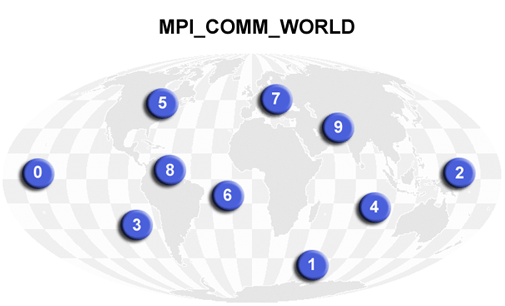
\includegraphics{MPI_COMM_WORLD.png}\hfill}

\begin{center}Figure 4: MPI\_COMM\_WORLD Obtained from computing.llnl.gov {[}2{]}
\end{center}
\textbf{Processes}: For this module, we just need to know that processes belong to the MPI\_COMM\_WORLD. If there are \emph{p} processes, then each process is defined by its rank, which starts from \emph{0} to \emph{p - 1}. The master has the rank \emph{0}.


\subsection{Some Common Functions:}
\label{introMPI/introMPI:some-common-functions}
The following functions are the functions that are commonly used in MPI programs:

\begin{Verbatim}[commandchars=\\\{\}]
MPI\_Init(\&argc, \&argv)
\end{Verbatim}

This function has to be called in every MPI program. It is used to initialize the MPI execution environment.

\begin{Verbatim}[commandchars=\\\{\}]
MPI\_Comm\_size(comm, \&size)
\end{Verbatim}

This function determines the number of processes in the communicator. The number of processes get store in the variable \emph{size}. All processes in a communicator have the same value of \emph{size}.

\begin{Verbatim}[commandchars=\\\{\}]
MPI\_Comm\_rank(comm, \&rank)
\end{Verbatim}

This function determines the rank of the calling process within the communicator. Each process is assigned uniquely by integer rank from \emph{0} to \emph{number of processes - 1}, and its rank gets stored in the variable \emph{rank}.

\begin{Verbatim}[commandchars=\\\{\}]
MPI\_Get\_processor\_name(name, \&len)
\end{Verbatim}

This function returns the unique processor name. Variable \emph{name} is the array of char for storing the name, and \emph{len} is the length of the name.

\begin{Verbatim}[commandchars=\\\{\}]
\PYG{n}{MPI\PYGZus{}Wtime}\PYG{p}{(}\PYG{p}{)}
\end{Verbatim}

This function returns an elapsed wall clock time in seconds on the calling processor. This function is often used to measure the running time of an MPI program. There is no defined starting point; therefore, in order to measure the running time, a programmer needs to call two different MPI\_Wtime(), and find the difference.

\begin{Verbatim}[commandchars=\\\{\}]
\PYG{n}{MPI\PYGZus{}Finalize}\PYG{p}{(}\PYG{p}{)}
\end{Verbatim}

This function terminates the MPI execution environment. MPI\_Finalize() has to be called by all processes before exiting.


\subsubsection{Example 1: Hello World MPI}
\label{introMPI/introMPI:example-1-hello-world-mpi}
\begin{Verbatim}[commandchars=\\\{\},numbers=left,firstnumber=1,stepnumber=1]
\PYG{c+cp}{\PYGZsh{}}\PYG{c+cp}{include \PYGZlt{}stdio.h\PYGZgt{}}
\PYG{c+cp}{\PYGZsh{}}\PYG{c+cp}{include \PYGZlt{}mpi.h\PYGZgt{}}

\PYG{k+kt}{int} \PYG{n+nf}{main} \PYG{p}{(}\PYG{k+kt}{int} \PYG{n}{argc}\PYG{p}{,} \PYG{k+kt}{char} \PYG{o}{*}\PYG{n}{argv}\PYG{p}{[}\PYG{p}{]}\PYG{p}{)} \PYG{p}{\PYGZob{}}
	\PYG{k+kt}{int} \PYG{n}{rank}\PYG{p}{,} \PYG{n}{nprocs}\PYG{p}{;}

	\PYG{n}{MPI\PYGZus{}Init} \PYG{p}{(}\PYG{o}{\PYGZam{}}\PYG{n}{argc}\PYG{p}{,} \PYG{o}{\PYGZam{}}\PYG{n}{argv}\PYG{p}{)}\PYG{p}{;}	\PYG{c+cm}{/* creates MPI execution environment */}
	\PYG{n}{MPI\PYGZus{}Comm\PYGZus{}rank} \PYG{p}{(}\PYG{n}{MPI\PYGZus{}COMM\PYGZus{}WORLD}\PYG{p}{,} \PYG{o}{\PYGZam{}}\PYG{n}{rank}\PYG{p}{)}\PYG{p}{;}	\PYG{c+cm}{/* get current process rank */}
	\PYG{n}{MPI\PYGZus{}Comm\PYGZus{}size} \PYG{p}{(}\PYG{n}{MPI\PYGZus{}COMM\PYGZus{}WORLD}\PYG{p}{,} \PYG{o}{\PYGZam{}}\PYG{n}{nprocs}\PYG{p}{)}\PYG{p}{;}\PYG{c+cm}{/* get number of processes */}
	\PYG{n}{printf}\PYG{p}{(}\PYG{l+s}{"}\PYG{l+s}{Hello world from process \PYGZpc{}d of \PYGZpc{}d}\PYG{l+s+se}{\PYGZbs{}n}\PYG{l+s}{"}\PYG{p}{,} \PYG{n}{rank}\PYG{p}{,} \PYG{n}{nprocs}\PYG{p}{)}\PYG{p}{;}
	\PYG{n}{MPI\PYGZus{}Finalize}\PYG{p}{(}\PYG{p}{)}\PYG{p}{;}			\PYG{c+cm}{/* terminates the MPI execution environment */}
	\PYG{k}{return} \PYG{l+m+mi}{0}\PYG{p}{;}
\PYG{p}{\PYGZcb{}}
\end{Verbatim}
\begin{quote}\begin{description}
\item[{Comments}] \leavevmode
In this hello world program, it illustrates how to use some basic functions of MPI. First, it initializes the MPI execution environment. Then it prints ``Hello world from process {[}rank{]} of {[}number of processes{]}''. Finally, it terminates the MPI execution environment.

\end{description}\end{quote}

You should eventually try to compile and run this code on your cluster account. Before that, we will explain a bit more about communication between processes, showing you another `Hello World' Example.  Then we will show you how to compile and run these programs.
\paragraph{References}


\chapter{MPI Communications}
\label{MPICommunication/MPICommunication:mpi-communications}\label{MPICommunication/MPICommunication::doc}

\section{Point-to-point Communication}
\label{MPICommunication/MPICommunication:point-to-point-communication}
Point-to-point communication is a way that pair of processors transmits the data between one another, one processor sending, and the other receiving. MPI provides SEND(MPI\_Send) and RECEIVE(MPI\_Recv) functions that allow point-to-point communication taking place in a communicator.

\begin{Verbatim}[commandchars=\\\{\}]
MPI\_Send(void* message, int count, MPI\_Datatype datatype, int destination, int tag, MPI\_Comm comm)

        - message:      initial address of the message
        - count:        number of entries to send
        - datatype:     type of each entry
        - destination:  rank of the receiving process
        - tag:          message tag is a way to identify the type of a message
        - comm:         communicator (MPI\_COMM\_WORLD)

MPI\_Recv(void* message, int count, MPI\_Datatype datatype, int source, int tag, MPI\_Comm comm, MPI\_Status *status)

        - source:       rank of the sending process
        - status:       return status
\end{Verbatim}

\begin{notice}{note}{Note:}
To read more on MPI\_Status, please read \href{http://www.netlib.org/utk/papers/mpi-book/node31.html}{MPI\_Status}.
\end{notice}


\subsection{MPI Datatype}
\label{MPICommunication/MPICommunication:mpi-datatype}
In most MPI functions, which you will be using, require you to specify the datatype of your message. Below is the table showing the corresponding datatype between MPI Datatype and C Datatype.

\begin{tabulary}{\linewidth}{|L|L|}
\hline
\textbf{
MPI Datatype
} & \textbf{
C Datatype
}\\\hline

MPI\_CHAR
 & 
signed char
\\\hline

MPI\_SHORT
 & 
signed short int
\\\hline

MPI\_INT
 & 
signed int
\\\hline

MPI\_LONG
 & 
signed long int
\\\hline

MPI\_UNSIGNED\_CHAR
 & 
unsigned char
\\\hline

MPI\_UNSIGNED\_SHORT
 & 
unsigned short int
\\\hline

MPI\_UNSIGNED
 & 
unsigned int
\\\hline

MPI\_UNSIGNED\_LONG
 & 
unsigned long int
\\\hline

MPI\_FLOAT
 & 
float
\\\hline

MPI\_DOUBLE
 & 
double
\\\hline

MPI\_LONG\_DOUBLE
 & 
long double
\\\hline
\end{tabulary}


\textbf{Table 1: Corresponding datatype between MPI and C}


\subsection{Example 2: Send and Receive Hello World}
\label{MPICommunication/MPICommunication:example-2-send-and-receive-hello-world}
\begin{Verbatim}[commandchars=\\\{\},numbers=left,firstnumber=1,stepnumber=1]
\PYG{c+cp}{\PYGZsh{}}\PYG{c+cp}{include \PYGZlt{}stdio.h\PYGZgt{}}
\PYG{c+cp}{\PYGZsh{}}\PYG{c+cp}{include "mpi.h"}

\PYG{c+cp}{\PYGZsh{}}\PYG{c+cp}{define FROM\PYGZus{}MASTER 1}

\PYG{k+kt}{int} \PYG{n+nf}{main}\PYG{p}{(}\PYG{k+kt}{int} \PYG{n}{argc}\PYG{p}{,} \PYG{k+kt}{char} \PYG{o}{*}\PYG{o}{*} \PYG{n}{argv}\PYG{p}{[}\PYG{p}{]}\PYG{p}{)} \PYG{p}{\PYGZob{}}

    \PYG{k+kt}{int} \PYG{n}{rank}\PYG{p}{,} \PYG{n}{nprocs}\PYG{p}{;}
    \PYG{k+kt}{char} \PYG{n}{message}\PYG{p}{[}\PYG{l+m+mi}{12}\PYG{p}{]} \PYG{o}{=} \PYG{l+s}{"}\PYG{l+s}{Hello, world}\PYG{l+s}{"}\PYG{p}{;}
    
    \PYG{c+cm}{/* status for MPI\PYGZus{}Recv */}
    \PYG{n}{MPI\PYGZus{}Status} \PYG{n}{status}\PYG{p}{;}
    
    \PYG{c+cm}{/* Initialize MPI execution environment */}
    \PYG{n}{MPI\PYGZus{}Init}\PYG{p}{(}\PYG{o}{\PYGZam{}}\PYG{n}{argc}\PYG{p}{,} \PYG{o}{\PYGZam{}}\PYG{n}{argv}\PYG{p}{)}\PYG{p}{;}
    \PYG{c+cm}{/* Determines the size of MPI\PYGZus{}COMM\PYGZus{}WORLD */}
    \PYG{n}{MPI\PYGZus{}Comm\PYGZus{}size}\PYG{p}{(}\PYG{n}{MPI\PYGZus{}COMM\PYGZus{}WORLD}\PYG{p}{,} \PYG{o}{\PYGZam{}}\PYG{n}{nprocs}\PYG{p}{)}
    \PYG{c+cm}{/* Give each process a unique rank */}
    \PYG{n}{MPI\PYGZus{}Comm\PYGZus{}rank}\PYG{p}{(}\PYG{n}{MPI\PYGZus{}COMM\PYGZus{}WORLD}\PYG{p}{,} \PYG{o}{\PYGZam{}}\PYG{n}{rank}\PYG{p}{)}\PYG{p}{;}
	
    \PYG{c+cm}{/* If the process is the master */}
    \PYG{k}{if} \PYG{p}{(} \PYG{n}{rank} \PYG{o}{=}\PYG{o}{=} \PYG{l+m+mi}{0} \PYG{p}{)}
        \PYG{c+cm}{/* Send message to process whose rank is 1 in the MPI\PYGZus{}COMM\PYGZus{}WORLD */}
        \PYG{n}{MPI\PYGZus{}Send}\PYG{p}{(}\PYG{o}{\PYGZam{}}\PYG{n}{message}\PYG{p}{,} \PYG{l+m+mi}{12}\PYG{p}{,} \PYG{n}{MPI\PYGZus{}CHAR}\PYG{p}{,} \PYG{l+m+mi}{1}\PYG{p}{,} \PYG{n}{FROM\PYGZus{}MASTER}\PYG{p}{,} \PYG{n}{MPI\PYGZus{}COMM\PYGZus{}WORLD}\PYG{p}{)}\PYG{p}{;}

    \PYG{c+cm}{/* If the process has rank of 1 */}
    \PYG{k}{else} \PYG{k}{if} \PYG{p}{(} \PYG{n}{rank} \PYG{o}{=}\PYG{o}{=} \PYG{l+m+mi}{1} \PYG{p}{)} \PYG{p}{\PYGZob{}}
        \PYG{c+cm}{/* Receive message sent from master */}
        \PYG{n}{MPI\PYGZus{}Recv}\PYG{p}{(}\PYG{o}{\PYGZam{}}\PYG{n}{message}\PYG{p}{,} \PYG{l+m+mi}{12}\PYG{p}{,} \PYG{n}{MPI\PYGZus{}CHAR}\PYG{p}{,} \PYG{l+m+mi}{0}\PYG{p}{,} \PYG{n}{FROM\PYGZus{}MASTER}\PYG{p}{,} \PYG{n}{MPI\PYGZus{}COMM\PYGZus{}WORLD}\PYG{p}{,} \PYG{o}{\PYGZam{}}\PYG{n}{status}\PYG{p}{)}\PYG{p}{;}
        \PYG{c+cm}{/* Print the rank and message */}
        \PYG{n}{printf}\PYG{p}{(}\PYG{l+s}{"}\PYG{l+s}{Process \PYGZpc{}d says : \PYGZpc{}s}\PYG{l+s+se}{\PYGZbs{}n}\PYG{l+s}{"}\PYG{p}{,} \PYG{n}{rank}\PYG{p}{,} \PYG{n}{message}\PYG{p}{)}\PYG{p}{;} 
    \PYG{p}{\PYGZcb{}}
    
    \PYG{c+cm}{/* Terminate MPI execution environment */}
    \PYG{n}{MPI\PYGZus{}Finalize}\PYG{p}{(}\PYG{p}{)}\PYG{p}{;}
\PYG{p}{\PYGZcb{}}
\end{Verbatim}
\begin{quote}\begin{description}
\item[{Comments}] \leavevmode
This MPI program illustrates the use of MPI\_Send and MPI\_Recv functions. Basically, the master sends a message, “Hello, world”, to the process whose rank is 1, and then after having received the message, the process prints the message along with its rank.

\end{description}\end{quote}


\section{Collective Communication}
\label{MPICommunication/MPICommunication:collective-communication}
Collective communication is a communication that must have all processes involved in the scope of a communicator. We will be using MPI\_COMM\_WORLD as our communicator; therefore, the collective communication will include all processes.

{\hfill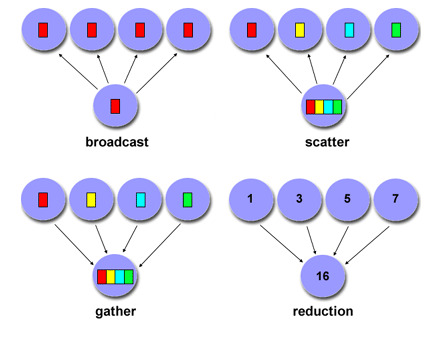
\includegraphics{collective.png}\hfill}

\begin{center}Figure 5: Collective Communications Obtained from computing.llnl.gov {[}1{]}
\end{center}
\begin{Verbatim}[commandchars=\\\{\}]
\PYG{n}{MPI\PYGZus{}Barrier}\PYG{p}{(}\PYG{n}{comm}\PYG{p}{)}
\end{Verbatim}

This function creates a barrier synchronization in a commmunicator(MPI\_COMM\_WORLD). Each task waits at MPI\_Barrier call until all other tasks in the communicator reach the same MPI\_Barrier call.

\begin{Verbatim}[commandchars=\\\{\}]
\PYG{n}{MPI\PYGZus{}Bcast}\PYG{p}{(}\PYG{o}{\PYGZam{}}\PYG{n}{message}\PYG{p}{,} \PYG{k+kt}{int} \PYG{n}{count}\PYG{p}{,} \PYG{n}{MPI\PYGZus{}Datatype} \PYG{n}{datatype}\PYG{p}{,} \PYG{k+kt}{int} \PYG{n}{root}\PYG{p}{,} \PYG{n}{comm}\PYG{p}{)}
\end{Verbatim}

This function displays the message to all other processes in MPI\_COMM\_WORLD from the process whose rank is root.

\begin{Verbatim}[commandchars=\\\{\}]
\PYG{n}{MPI\PYGZus{}Reduce}\PYG{p}{(}\PYG{o}{\PYGZam{}}\PYG{n}{message}\PYG{p}{,} \PYG{o}{\PYGZam{}}\PYG{n}{receivemessage}\PYG{p}{,} \PYG{k+kt}{int} \PYG{n}{count}\PYG{p}{,} \PYG{n}{MPI\PYGZus{}Datatype} \PYG{n}{datatype}\PYG{p}{,} \PYG{n}{MPI\PYGZus{}Op} \PYG{n}{op}\PYG{p}{,} \PYG{k+kt}{int} \PYG{n}{root}\PYG{p}{,} \PYG{n}{comm}\PYG{p}{)}
\end{Verbatim}

This function applies a reduction operation on all tasks in MPI\_COMM\_WORLD and reduces results from each process into one value. MPI\_Op includes for example, MPI\_MAX, MPI\_MIN, MPI\_PROD, and MPI\_SUM, etc.
\begin{quote}

\begin{notice}{note}{Note:}
To read more on MPI\_Op, please read \href{http://www.mpi-forum.org/docs/mpi-11-html/node78.html\#Node78}{MPI\_Op}.
\end{notice}
\end{quote}

\begin{Verbatim}[commandchars=\\\{\}]
\PYG{n}{MPI\PYGZus{}Scatter}\PYG{p}{(}\PYG{o}{\PYGZam{}}\PYG{n}{message}\PYG{p}{,} \PYG{k+kt}{int} \PYG{n}{count}\PYG{p}{,} \PYG{n}{MPI\PYGZus{}Datatype}\PYG{p}{,} \PYG{o}{\PYGZam{}}\PYG{n}{receivemessage}\PYG{p}{,} \PYG{k+kt}{int} \PYG{n}{count}\PYG{p}{,} \PYG{n}{MPI\PYGZus{}Datatype}\PYG{p}{,} \PYG{k+kt}{int} \PYG{n}{root}\PYG{p}{,} \PYG{n}{comm}\PYG{p}{)}
\end{Verbatim}

This function divides a message into equal contiguous parts and sends each part to each node. The master gets the first part, and the process whose rank is 1 gets the second part, and so on. The number of elements get sent to each worker is specified by count.

\begin{Verbatim}[commandchars=\\\{\}]
\PYG{n}{MPI\PYGZus{}Gather}\PYG{p}{(}\PYG{o}{\PYGZam{}}\PYG{n}{message}\PYG{p}{,} \PYG{k+kt}{int} \PYG{n}{count}\PYG{p}{,} \PYG{n}{MPI\PYGZus{}Datatype}\PYG{p}{,} \PYG{o}{\PYGZam{}}\PYG{n}{receivemessage}\PYG{p}{,} \PYG{k+kt}{int} \PYG{n}{count}\PYG{p}{,} \PYG{n}{MPI\PYGZus{}Datatype}\PYG{p}{,} \PYG{k+kt}{int} \PYG{n}{root}\PYG{p}{,} \PYG{n}{comm}\PYG{p}{)}
\end{Verbatim}

This function collects distinct messages from each task in the communicator to a single task. This function is the reverse operation of MPI\_Scatter.


\section{Let's Try It}
\label{MPICommunication/MPICommunication:let-s-try-it}
In the next section we will describe how to compile and run these examples so that you can try them.
\paragraph{References}


\chapter{Compiling and First Two Activites}
\label{CompileAndActivity/compileandactivity::doc}\label{CompileAndActivity/compileandactivity:compiling-and-first-two-activites}

\section{Compiling an MPI program}
\label{CompileAndActivity/compileandactivity:compiling-an-mpi-program}
To compile an MPI program on your local cluster, you can enter the following commands in the terminal:

First, we need to make an executable file from the MPI program by using \textbf{mpicc}:

\begin{Verbatim}[commandchars=\\\{\}]
\PYG{n}{mpicc} \PYG{o}{-}\PYG{n}{o} \PYG{n}{filename} \PYG{n}{filename}\PYG{p}{.}\PYG{n}{c}
\end{Verbatim}

Then you are able to execute it using \textbf{mpirun} :

\begin{Verbatim}[commandchars=\\\{\}]
mpirun -machinefile machines -np \#processes ./filename
\end{Verbatim}

\begin{notice}{note}{Note:}
\textbf{machines}: is the instruction for running the executable file on a cluster. It tells the executable file to run on which nodes and how many times on those nodes. For example, machines on LittleFe has structure as follow:
\begin{itemize}
\item {} 
node000.bccd.net    slots = 1

\item {} 
node011.bccd.net    slots = 1

\item {} 
node012.bccd.net    slots = 1

\item {} 
node013.bccd.net    slots = 1

\item {} 
node014.bccd.net    slots = 1

\item {} 
node015.bccd.net    slots = 1

\end{itemize}
\end{notice}

Moreover, you can also compile an MPI program without using \textbf{machines}, you can use the following command to run only on the master node:

\begin{Verbatim}[commandchars=\\\{\}]
mpirun -np \#processes ./filename
\end{Verbatim}

\begin{notice}{note}{Note:}
Please ask your instructor for instructions on how to log in onto your local machine.
\end{notice}


\section{Try the simple examples}
\label{CompileAndActivity/compileandactivity:try-the-simple-examples}
Log into your cluster and make sure that you have the following example files in your account:

Simplest Hello World Example:
\code{download hellompi.c}

Hello World by Sending messages:
\code{download example2.c}

You can specifically compile the simplest example like this:

\begin{Verbatim}[commandchars=\\\{\}]
\PYG{n}{mpicc} \PYG{o}{-}\PYG{n}{o} \PYG{n}{hellompi} \PYG{n}{hellompi}\PYG{p}{.}\PYG{n}{c}
\end{Verbatim}

To run it on your cluster using 3 processes, you can do this, assuming you also have a
file called machines that describes your system:

\begin{Verbatim}[commandchars=\\\{\}]
\PYG{n}{mpirun} \PYG{o}{-}\PYG{n}{machinefile} \PYG{n}{machines} \PYG{o}{-}\PYG{n}{np} \PYG{l+m+mi}{3} \PYG{p}{.}\PYG{o}{/}\PYG{n}{hellompi}
\end{Verbatim}

Sepending on how many other people are using your cluster and how big it is, you can try
different numbers of processes by changing the 3 above.

Once that seems to be working for you, try the exammple 2, which uses sends and receives.

\begin{notice}{note}{Note:}
The procedure for compiling and running all of your mpi code will follow this format.
\end{notice}


\section{Activity 1: Computing ${\pi}$ ?}
\label{CompileAndActivity/compileandactivity:activity-1-computing}
Download the source code to do this activity:
\code{download mpi\_pi\_todo.c}

Have it open in an editor so that you can work on it.  Or at a minimum use your browser and right-click on the link above and choose to open it in a new browser window.

In this activity, we are going to compute ${\pi}$ using integration. We have formula:
\begin{gather}
\begin{split}\int_0^1 \frac{4}{1 + x^2} dx = {\pi}\end{split}\notag
\end{gather}
Therefore, we can compute the area under the curve to get the value of the integral.

{\hfill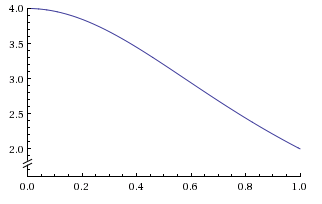
\includegraphics{graph.png}\hfill}

\begin{center}Figure 4: Graph for function
\end{center}\begin{quote}\begin{description}
\item[{Comments}] \leavevmode\begin{itemize}
\item {} 
We can split the area under the curve into bins. The idea is to group the bins into smaller chunks, and so we can use each process to calculate each chunk, and then combine the result into one value. Remember, that we can get a more accurate result if you split the area under the curve into more number of bins.

\item {} 
In this activity, we also want you to time your computation by using MPI\_Wtime() function. We provide you some parts of the code, and would like you to complete \textbf{TO DO}, and then you can experiment with the different number of bins you are using. Moreover,  we want you to execute your program with different number of processes, and compare your timings. We will walk you through the code step by step.

\item {} 
First, you need to initialize the MPI execution environment, define the size of communicator, and define the rank of each process. This should be straight forward for you. You are asked to complete this task.

\item {} 
Then you want to let each process know the \textbf{number of bins} you are using. Therefore, you need to broadcast the \textbf{number of bins} to all processes in our MPI\_COMM\_WORLD. You should use \textbf{MPI\_Bcast} to broadcast the \textbf{number of bins}. You are asked to complete this part of the code.

\item {} 
Now we are ready to ask each process compute their task. We want to evaluate the integral of $\frac {4}{1 + x^2}$ from \emph{0} to \emph{1}, and we can do so by finding the sum of all bins from \emph{0} to \emph{1}. Each bin is approximately $\frac {1}{n} * \frac {4}{1 + x^2}$ (\textbf{n} is the number of bins). We are iterating over the number of bins, and we start from \emph{0}; therefore, to find the center of each bin, we need to add \emph{+ 0.5} to variable \emph{i}. Moreover, in the \textbf{for loop}, we ask the rank \emph{0} to compute the first bin, the (nprocs) bin, and so on, rank \emph{1} to compute the second bin, the (nprocs + 1) bin, and so on, ..., as long as value of \emph{i} is less than \textbf{n}. Suppose that there are \emph{p} processes, then these \emph{p} processes will take the first \emph{p} bins, where process whose rank is 0 takes \emph{1st} bin, process whose rank is 1 takes \emph{2nd} bin, and so on. If there are any bins left, process whose rank is 1 takes \emph{pth} bin, and so on. This can be done by using the following piece of code:

\begin{Verbatim}[commandchars=\\\{\}]
\PYG{c+cm}{/* Calculating for each process */}
\PYG{n}{step} \PYG{o}{=} \PYG{l+m+mf}{1.0} \PYG{o}{/} \PYG{p}{(}\PYG{k+kt}{double}\PYG{p}{)} \PYG{n}{n}\PYG{p}{;}
\PYG{n}{sum} \PYG{o}{=} \PYG{l+m+mf}{0.0}\PYG{p}{;}
\PYG{k}{for} \PYG{p}{(}\PYG{n}{i} \PYG{o}{=} \PYG{n}{rank}\PYG{p}{;} \PYG{n}{i} \PYG{o}{\PYGZlt{}} \PYG{n}{n}\PYG{p}{;} \PYG{n}{i} \PYG{o}{+}\PYG{o}{=} \PYG{n}{nprocs}\PYG{p}{)} \PYG{p}{\PYGZob{}}
    \PYG{n}{x} \PYG{o}{=} \PYG{n}{step} \PYG{o}{*} \PYG{p}{(}\PYG{p}{(}\PYG{k+kt}{double}\PYG{p}{)}\PYG{n}{i} \PYG{o}{+} \PYG{l+m+mf}{0.5}\PYG{p}{)}\PYG{p}{;}
    \PYG{n}{sum} \PYG{o}{+}\PYG{o}{=} \PYG{p}{(}\PYG{l+m+mf}{4.0}\PYG{o}{/}\PYG{p}{(}\PYG{l+m+mf}{1.0} \PYG{o}{+} \PYG{n}{x}\PYG{o}{*}\PYG{n}{x}\PYG{p}{)}\PYG{p}{)}\PYG{p}{;}
\PYG{p}{\PYGZcb{}}

\PYG{n}{mypi} \PYG{o}{=} \PYG{n}{step} \PYG{o}{*} \PYG{n}{sum}\PYG{p}{;}
\end{Verbatim}

\item {} 
When all processes have finished their computations, their results are stored in \textbf{mypi}. Therefore, we can reduce all their results into one result, which is the value of ${\pi}$. Your task is to complete this part by using MPI\_Reduce.

\end{itemize}

\end{description}\end{quote}

If you get stuck and want to move on, download the entire source code (originally from www.mcs.anl.gov {[}1{]}):
\code{download mpi\_pi\_done.c}


\section{Activity 2: Vector Matrix Multiplication}
\label{CompileAndActivity/compileandactivity:activity-2-vector-matrix-multiplication}
To download the source code to do this activity:
\code{download vector\_matrix\_todo.c}

Have it open in an editor so that you can work on it.  Or at a minimum use your browser and right-click on the link above and choose to open it in a new browser window.

In this activity, we are going to compute vector matrix multiplication. This activity illustrates the use of MPI\_Bcast, MPI\_Scatter, and MPI\_Gather to do this multiplication. First, we want you to complete this MPI program by filling codes at \textbf{TO DO}. After having completed this task, try to run this MPI program by using different number of processes. Try to explain to yourself what is happening !

Here is how the vector matrix multiplication works. First, let's say we have a matrix \emph{A}, and a vector \emph{x} as below:

{\hfill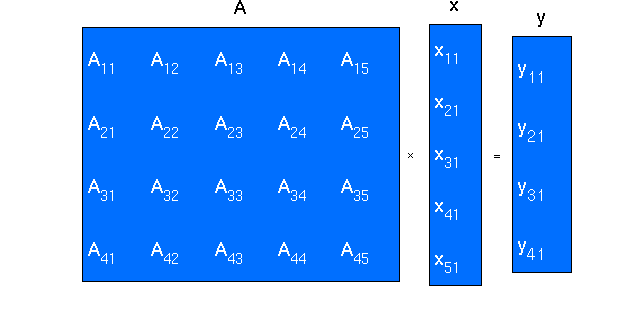
\includegraphics{vector_matrix_multi.png}\hfill}

\begin{center}Figure 5: vector matrix multiplication Obtained from cms.uni-konstanz.de {[}2{]}
\end{center}
This multiplication produces a new vector whose length is the number of rows of matrix \emph{A}. The multiplication is very simple. We take a row of matrix \emph{A} dot product with vector \emph{x}, and this produces an element of the result vector. For instance, the first row of matrix \emph{A} dot products with vector \emph{x} will produce the first element in vector \emph{y}.
\begin{quote}\begin{description}
\item[{Comments}] \leavevmode\begin{itemize}
\item {} 
We will step you through this activity step by step. Since this is an MPI program, we need to create the MPI execution environment, define the size of the communicator, and give each process a unique rank. You are asked to completed this part of the code.

\item {} 
After having initialized the MPI environment, we want to ask the master to initialize the vector and matrix we are going to multiply. In order to do that, we check if the process is master. If so, we initialize the matrix and vector. We initialize every entry to 1 because of its simplicity.

\begin{Verbatim}[commandchars=\\\{\}]
\PYG{k}{if} \PYG{p}{(}\PYG{n}{rank} \PYG{o}{=}\PYG{o}{=} \PYG{l+m+mi}{0}\PYG{p}{)} \PYG{p}{\PYGZob{}}
    \PYG{c+cm}{/* Initialize the matrix and vector */}
    \PYG{k}{for}\PYG{p}{(}\PYG{n}{i}\PYG{o}{=}\PYG{l+m+mi}{0}\PYG{p}{;} \PYG{n}{i} \PYG{o}{\PYGZlt{}} \PYG{n}{WIDTH}\PYG{p}{;} \PYG{n}{i}\PYG{o}{+}\PYG{o}{+}\PYG{p}{)} \PYG{p}{\PYGZob{}}
        \PYG{n}{vector}\PYG{p}{[}\PYG{n}{i}\PYG{p}{]} \PYG{o}{=} \PYG{l+m+mi}{1}\PYG{p}{;}
        \PYG{k}{for}\PYG{p}{(}\PYG{n}{j} \PYG{o}{=} \PYG{l+m+mi}{0}\PYG{p}{;} \PYG{n}{j} \PYG{o}{\PYGZlt{}} \PYG{n}{WIDTH}\PYG{p}{;} \PYG{n}{j}\PYG{o}{+}\PYG{o}{+}\PYG{p}{)} \PYG{p}{\PYGZob{}}
            \PYG{n}{matrix}\PYG{p}{[}\PYG{n}{i}\PYG{p}{]}\PYG{p}{[}\PYG{n}{j}\PYG{p}{]} \PYG{o}{=} \PYG{l+m+mi}{1}\PYG{p}{;}
        \PYG{p}{\PYGZcb{}}
    \PYG{p}{\PYGZcb{}}
\PYG{p}{\PYGZcb{}}
\end{Verbatim}

\item {} 
Since the vector is not very large and all processes must have this vector to do the multiplication, we will broadcast the entire vector to all processes. We do this by using MPI\_Bcast. In addition, we want to distribute the matrix to each process in the MPI\_COMM\_WORLD. We would do this using MPI\_Scatter. You are asked to complete this task.

\item {} 
When all processes can see the vector and some rows of matrix, they are now able to do the multiplication. We need to store their result in the result vector.

\begin{Verbatim}[commandchars=\\\{\}]
\PYG{k}{for}\PYG{p}{(}\PYG{n}{i} \PYG{o}{=} \PYG{l+m+mi}{0}\PYG{p}{;} \PYG{n}{i} \PYG{o}{\PYGZlt{}} \PYG{n}{chunk\PYGZus{}size}\PYG{p}{;} \PYG{n}{i}\PYG{o}{+}\PYG{o}{+}\PYG{p}{)} \PYG{p}{\PYGZob{}}
    \PYG{n}{result}\PYG{p}{[}\PYG{n}{i}\PYG{p}{]} \PYG{o}{=} \PYG{l+m+mi}{0}\PYG{p}{;}
    \PYG{k}{for}\PYG{p}{(}\PYG{n}{j} \PYG{o}{=} \PYG{l+m+mi}{0}\PYG{p}{;} \PYG{n}{j} \PYG{o}{\PYGZlt{}} \PYG{n}{WIDTH}\PYG{p}{;} \PYG{n}{j}\PYG{o}{+}\PYG{o}{+}\PYG{p}{)} \PYG{p}{\PYGZob{}}
        \PYG{n}{result}\PYG{p}{[}\PYG{n}{i}\PYG{p}{]} \PYG{o}{+}\PYG{o}{=} \PYG{n}{local\PYGZus{}matrix}\PYG{p}{[}\PYG{n}{i}\PYG{p}{]}\PYG{p}{[}\PYG{n}{j}\PYG{p}{]} \PYG{o}{*} \PYG{n}{vector}\PYG{p}{[}\PYG{n}{j}\PYG{p}{]}\PYG{p}{;}
    \PYG{p}{\PYGZcb{}}
\PYG{p}{\PYGZcb{}}
\end{Verbatim}

\item {} 
The last part you need to complete is to gather all result vectors in all processes, and store them in the output vector, called global\_result vector. This will be our result vector. Moreover, we can print out the value of each element in the global\_result vector, and then terminate the MPI execution environment.

\end{itemize}

\end{description}\end{quote}

If you get stuck and wanto move on, download the entire source code (originally from www.public.asu.edu/\textasciitilde{}dstanzoi {[}3{]}):
\code{download vector\_matrix\_done.c}
\paragraph{References}


\chapter{Decomposition and Two Advanced Activities}
\label{DecompositionAndActivity/DecompositionAndActivity::doc}\label{DecompositionAndActivity/DecompositionAndActivity:decomposition-and-two-advanced-activities}
Decomposition is a very important aspect of many parallel programs. Decomposition is a way to divide up the taske fairly across the data you need to compute over or the computation to be performed; thus, each task can be distributed to each process. There are many ways to break up a large task into smaller tasks, and you should choose the way that the best suits your problem. For instance, you might guess that splitting your matrix by rows and having each process work on a set of rows will work best for matrix multiplication. Below is an example of a decomposition method. You will see this type of pattern very often in parallel code.


\section{Example 3: Decompose the matrix by row}
\label{DecompositionAndActivity/DecompositionAndActivity:example-3-decompose-the-matrix-by-row}
\begin{Verbatim}[commandchars=\\\{\}]
\PYG{n}{averow} \PYG{o}{=} \PYG{n}{ROW}\PYG{o}{/}\PYG{n}{numworkers}\PYG{p}{;}
\PYG{n}{extra} \PYG{o}{=} \PYG{n}{ROW}\PYG{o}{\PYGZpc{}}\PYG{n}{numworkers}\PYG{p}{;}
\PYG{n}{offset} \PYG{o}{=} \PYG{l+m+mi}{0}\PYG{p}{;}
\PYG{n}{mtype} \PYG{o}{=} \PYG{n}{FROM\PYGZus{}MASTER}\PYG{p}{;}

\PYG{k}{for} \PYG{p}{(}\PYG{n}{dest} \PYG{o}{=} \PYG{l+m+mi}{1}\PYG{p}{;} \PYG{n}{dest} \PYG{o}{\PYGZlt{}}\PYG{o}{=} \PYG{n}{numworkers}\PYG{p}{;} \PYG{n}{dest}\PYG{o}{+}\PYG{o}{+}\PYG{p}{)} \PYG{p}{\PYGZob{}}
    \PYG{n}{rows} \PYG{o}{=} \PYG{p}{(}\PYG{n}{dest} \PYG{o}{\PYGZlt{}}\PYG{o}{=} \PYG{n}{extra}\PYG{p}{)} \PYG{o}{?} \PYG{n}{averow} \PYG{o}{+} \PYG{l+m+mi}{1} \PYG{o}{:} \PYG{n}{averow}\PYG{p}{;}
    \PYG{c+c1}{// Then send to each worker the number of rows}
\end{Verbatim}
\begin{quote}\begin{description}
\item[{Comments}] \leavevmode\begin{itemize}
\item {} 
\textbf{rows = (dest \textless{}= extra) ? averow + 1 : averow} means if \textbf{dest \textless{}= extra}, we have \textbf{rows = averow + 1}. Otherwise, we have \textbf{rows = averow}. This is a shorter version of if and else statement.

\item {} 
In this example, \textbf{ROW} is the number of rows of the matrix, so each process will get at least \textbf{averow} rows. The \textbf{extra} is the extra rows when \textbf{ROW} is not divisible by number of workers. In order to send each task to each worker, we need to iterate over the number of workers. Then if we have extra rows, we know that number of extra rows must be less than the number of workers, so we can give one more row to workers whose ranks are less than or equal to extra.

\end{itemize}

\end{description}\end{quote}


\subsection{Activity 3: Vector Matrix Multiplication Improved Version}
\label{DecompositionAndActivity/DecompositionAndActivity:activity-3-vector-matrix-multiplication-improved-version}
To download the source code to do this activity:
\code{download vector\_matrix\_todo.c}

Have it open in an editor so that you can work on it.  Or at a minimum use your browser and right-click on the link above and choose to open it in a new browser window.

In this activity, we will be using decomposition technique, MPI\_Send, and MPI\_Recv to
improve the efficiency and accuracy of vector matrix multiplication. We already seen that by using
MPI\_Scatter, we do not get the right result if the length of vector is not divisible by
the number of workers. Thus, we want to use the decomposition technique to help us divide
the task fairly among each worker. Then, we can send each task to each worker by using MPI\_Send.
After the workers having received their tasks, they will compute their own task, and send their results
back to the master. Finally the master will receive results from workers, and combine them into a result vector.
\begin{quote}\begin{description}
\item[{Comments}] \leavevmode\begin{itemize}
\item {} 
I will walk you through the code step by step. First, we will need to initialize the MPI environment, define the size of the communicator, and give a rank to each process. This should be straight forward to you because you have seen this many times already.

\begin{Verbatim}[commandchars=\\\{\}]
\PYG{c+cm}{/* Initialize MPI execution environment */}
\PYG{n}{MPI\PYGZus{}Init}\PYG{p}{(} \PYG{o}{\PYGZam{}}\PYG{n}{argc}\PYG{p}{,}\PYG{o}{\PYGZam{}}\PYG{n}{argv}\PYG{p}{)}\PYG{p}{;}
\PYG{n}{MPI\PYGZus{}Comm\PYGZus{}rank}\PYG{p}{(} \PYG{n}{MPI\PYGZus{}COMM\PYGZus{}WORLD}\PYG{p}{,} \PYG{o}{\PYGZam{}}\PYG{n}{rank}\PYG{p}{)}\PYG{p}{;}
\PYG{n}{MPI\PYGZus{}Comm\PYGZus{}size}\PYG{p}{(} \PYG{n}{MPI\PYGZus{}COMM\PYGZus{}WORLD}\PYG{p}{,} \PYG{o}{\PYGZam{}}\PYG{n}{nprocs}\PYG{p}{)}\PYG{p}{;}
\end{Verbatim}

\item {} 
Then we want to initialize the vector and matrix on master node. This can be done by:

\begin{Verbatim}[commandchars=\\\{\}]
\PYG{k}{if} \PYG{p}{(}\PYG{n}{rank} \PYG{o}{=}\PYG{o}{=} \PYG{l+m+mi}{0}\PYG{p}{)} \PYG{p}{\PYGZob{}}
    \PYG{c+cm}{/* Initialize Matrix and Vector */}
    \PYG{k}{for}\PYG{p}{(}\PYG{n}{i} \PYG{o}{=} \PYG{l+m+mi}{0}\PYG{p}{;} \PYG{n}{i} \PYG{o}{\PYGZlt{}} \PYG{n}{WIDTH}\PYG{p}{;} \PYG{n}{i}\PYG{o}{+}\PYG{o}{+}\PYG{p}{)} \PYG{p}{\PYGZob{}}
    \PYG{n}{vector}\PYG{p}{[}\PYG{n}{i}\PYG{p}{]} \PYG{o}{=} \PYG{l+m+mi}{1}\PYG{p}{;}
        \PYG{k}{for}\PYG{p}{(}\PYG{n}{j} \PYG{o}{=} \PYG{l+m+mi}{0}\PYG{p}{;} \PYG{n}{j} \PYG{o}{\PYGZlt{}} \PYG{n}{WIDTH}\PYG{p}{;} \PYG{n}{j}\PYG{o}{+}\PYG{o}{+}\PYG{p}{)} \PYG{p}{\PYGZob{}}
            \PYG{n}{matrix}\PYG{p}{[}\PYG{n}{i}\PYG{p}{]}\PYG{p}{[}\PYG{n}{j}\PYG{p}{]} \PYG{o}{=} \PYG{l+m+mi}{1}\PYG{p}{;}
        \PYG{p}{\PYGZcb{}}
    \PYG{p}{\PYGZcb{}}
\PYG{p}{\PYGZcb{}}
\end{Verbatim}

\item {} 
We have seen that using the collective communications without decomposition is not the best way of doing this problem. Here is a better way that will work for any number of processes. We will be using the decomposition technique above to split the task for each process. Then, the master will be sending each process the number of rows (\textbf{rows}) of matrix, and the vector. You are asked to complete this part of the code.

\item {} 
\begin{notice}{note}{Note:}
You should use MPI\_Send to send the starting rows, and number of rows, and some rows of matrix, and the vector to the workers. Moreover, when you send some rows of matrix, you should use MPI\_Send(\&matrix{[}starting row{]}{[}0{]}, number of elements, ...). This will send the rows of matrix, which contain the number of elements, and it starts from the first element in that row.
\end{notice}

\item {} 
\begin{Verbatim}[commandchars=\\\{\}]
\PYG{n}{averow} \PYG{o}{=} \PYG{n}{ROW}\PYG{o}{/}\PYG{n}{numworkers}\PYG{p}{;}
\PYG{n}{extra} \PYG{o}{=} \PYG{n}{ROW}\PYG{o}{\PYGZpc{}}\PYG{n}{numworkers}\PYG{p}{;}
\PYG{n}{offset} \PYG{o}{=} \PYG{l+m+mi}{0}\PYG{p}{;}
\PYG{n}{mtype} \PYG{o}{=} \PYG{n}{FROM\PYGZus{}MASTER}\PYG{p}{;}

\PYG{k}{for} \PYG{p}{(}\PYG{n}{dest} \PYG{o}{=} \PYG{l+m+mi}{1}\PYG{p}{;} \PYG{n}{dest} \PYG{o}{\PYGZlt{}}\PYG{o}{=} \PYG{n}{numworkers}\PYG{p}{;} \PYG{n}{dest}\PYG{o}{+}\PYG{o}{+}\PYG{p}{)} \PYG{p}{\PYGZob{}}
    \PYG{n}{rows} \PYG{o}{=} \PYG{p}{(}\PYG{n}{dest} \PYG{o}{\PYGZlt{}}\PYG{o}{=} \PYG{n}{extra}\PYG{p}{)} \PYG{o}{?} \PYG{n}{averow} \PYG{o}{+} \PYG{l+m+mi}{1} \PYG{o}{:} \PYG{n}{averow}\PYG{p}{;}
    \PYG{c+c1}{// TO DO}
    \PYG{p}{.}\PYG{p}{.}\PYG{p}{.}\PYG{p}{.}\PYG{p}{.}\PYG{p}{.}\PYG{p}{.}\PYG{p}{.}\PYG{p}{.}\PYG{p}{.}\PYG{p}{.}\PYG{p}{.}\PYG{p}{.}\PYG{p}{.}
    \PYG{c+c1}{// end TO DO}
\PYG{p}{\PYGZcb{}}
\end{Verbatim}

\item {} 
After having sent the messages to all workers, we need to ask workers to receive the messages from the master. We check if the process is not the master, we will use MPI\_Recv to receive the messages sent from the master. You are asked complete this task.

\begin{Verbatim}[commandchars=\\\{\}]
\PYG{k}{if} \PYG{p}{(}\PYG{n}{rank} \PYG{o}{\PYGZgt{}} \PYG{l+m+mi}{0}\PYG{p}{)} \PYG{p}{\PYGZob{}}
    \PYG{n}{mtype} \PYG{o}{=} \PYG{n}{FROM\PYGZus{}MASTER}\PYG{p}{;}
    \PYG{c+cm}{/* Receive the task from master */}
    \PYG{c+c1}{// TO DO:}
    \PYG{p}{.}\PYG{p}{.}\PYG{p}{.}\PYG{p}{.}\PYG{p}{.}\PYG{p}{.}\PYG{p}{.}\PYG{p}{.}\PYG{p}{.}\PYG{p}{.}\PYG{p}{.}\PYG{p}{.}\PYG{p}{.}\PYG{p}{.}
    \PYG{c+c1}{// end TO DO}
\PYG{p}{\PYGZcb{}}
\end{Verbatim}

\item {} 
Each worker now can compute their task, and then we have to send the results back to the master. Sending results back to master should not be difficult. Since result is just a vector, we can send the starting rows, number of rows, and entire result vector to the master. You are asked to complete this part.

\begin{Verbatim}[commandchars=\\\{\}]
\PYG{c+cm}{/* Each worker works on their computation */}
\PYG{k}{for}\PYG{p}{(}\PYG{n}{i} \PYG{o}{=} \PYG{l+m+mi}{0}\PYG{p}{;} \PYG{n}{i} \PYG{o}{\PYGZlt{}} \PYG{n}{rows}\PYG{p}{;} \PYG{n}{i}\PYG{o}{+}\PYG{o}{+}\PYG{p}{)} \PYG{p}{\PYGZob{}}
    \PYG{n}{result}\PYG{p}{[}\PYG{n}{i}\PYG{p}{]} \PYG{o}{=} \PYG{l+m+mi}{0}\PYG{p}{;}
    \PYG{k}{for}\PYG{p}{(}\PYG{n}{j} \PYG{o}{=} \PYG{l+m+mi}{0}\PYG{p}{;} \PYG{n}{j} \PYG{o}{\PYGZlt{}} \PYG{n}{WIDTH}\PYG{p}{;} \PYG{n}{j}\PYG{o}{+}\PYG{o}{+}\PYG{p}{)} \PYG{p}{\PYGZob{}}
        \PYG{n}{result}\PYG{p}{[}\PYG{n}{i}\PYG{p}{]} \PYG{o}{+}\PYG{o}{=} \PYG{n}{matrix}\PYG{p}{[}\PYG{n}{i}\PYG{p}{]}\PYG{p}{[}\PYG{n}{j}\PYG{p}{]} \PYG{o}{*} \PYG{n}{vector}\PYG{p}{[}\PYG{n}{j}\PYG{p}{]}\PYG{p}{;}
    \PYG{p}{\PYGZcb{}}
\PYG{p}{\PYGZcb{}}

\PYG{c+cm}{/* send the result back to the master */}
\PYG{n}{mtype} \PYG{o}{=} \PYG{n}{FROM\PYGZus{}WORKER}\PYG{p}{;}
\PYG{c+c1}{// TO DO:}
\PYG{c+c1}{//............}
\PYG{c+c1}{//end TO DO}
\end{Verbatim}

\item {} 
Finally, the master has to receive the results from all workers. You are asked to complete this task.

\begin{Verbatim}[commandchars=\\\{\}]
\PYG{c+cm}{/* Receiving the work from each worker */}
\PYG{n}{mtype} \PYG{o}{=} \PYG{n}{FROM\PYGZus{}WORKER}\PYG{p}{;}
\PYG{k}{for} \PYG{p}{(}\PYG{n}{i} \PYG{o}{=} \PYG{l+m+mi}{1}\PYG{p}{;} \PYG{n}{i} \PYG{o}{\PYGZlt{}}\PYG{o}{=} \PYG{n}{numworkers}\PYG{p}{;} \PYG{n}{i}\PYG{o}{+}\PYG{o}{+}\PYG{p}{)} \PYG{p}{\PYGZob{}}
    \PYG{n}{source} \PYG{o}{=} \PYG{n}{i}\PYG{p}{;}
    \PYG{c+c1}{// TO DO}
    \PYG{c+c1}{//..............}
    \PYG{c+c1}{// end TO DO}
    \PYG{n}{printf}\PYG{p}{(}\PYG{l+s}{"}\PYG{l+s}{Received results from task \PYGZpc{}d}\PYG{l+s+se}{\PYGZbs{}n}\PYG{l+s}{"}\PYG{p}{,} \PYG{n}{source}\PYG{p}{)}\PYG{p}{;}
\PYG{p}{\PYGZcb{}}
\end{Verbatim}

\end{itemize}

\end{description}\end{quote}

To download the entire source code (if you get stuck):
\code{download vector\_matrix\_done.c}


\subsection{Activity 4: Matrix Multiplication}
\label{DecompositionAndActivity/DecompositionAndActivity:activity-4-matrix-multiplication}
Download the source code to do this activity:
\code{download matrix\_multiplication\_todo.c}

Have it open in an editor so that you can work on it.  Or at a minimum use your browser and right-click on the link above and choose to open it in a new browser window.

In this activity, we want you to use decomposition technique, MPI\_Send, and MPI\_Recv in previous activities to complete the matrix multiplication program. If you have not seen matrix multiplication before, please click on \href{http://mathworld.wolfram.com/MatrixMultiplication.html}{matrix multiplication} to read how matrix multiplication works.
\begin{quote}\begin{description}
\item[{Comments}] \leavevmode\begin{itemize}
\item {} 
This activity is not much different from the previous activity. First, we use the decomposition method in the previous activity. Then we want to send some rows from the first matrix, and entire second matrix to each worker. Note that this is not the most efficient method of doing matrix multiplication because when the second matrix gets really large, we might not be able to send entire matrix to each worker. We use this method because of its simplicity.

\begin{Verbatim}[commandchars=\\\{\}]
\PYG{c+cm}{/* Computing the row and extra row */}
\PYG{n}{averow} \PYG{o}{=} \PYG{n}{ROWA}\PYG{o}{/}\PYG{n}{numworkers}\PYG{p}{;}
\PYG{n}{extra} \PYG{o}{=} \PYG{n}{ROWA}\PYG{o}{\PYGZpc{}}\PYG{n}{numworkers}\PYG{p}{;}
\PYG{n}{offset} \PYG{o}{=} \PYG{l+m+mi}{0}\PYG{p}{;}
\PYG{n}{mtype} \PYG{o}{=} \PYG{n}{FROM\PYGZus{}MASTER}\PYG{p}{;}

\PYG{c+cm}{/* Distributing the task to each worker */}
\PYG{k}{for} \PYG{p}{(}\PYG{n}{dest} \PYG{o}{=} \PYG{l+m+mi}{1}\PYG{p}{;} \PYG{n}{dest} \PYG{o}{\PYGZlt{}}\PYG{o}{=} \PYG{n}{numworkers}\PYG{p}{;} \PYG{n}{dest}\PYG{o}{+}\PYG{o}{+}\PYG{p}{)} \PYG{p}{\PYGZob{}}
    \PYG{c+cm}{/*If the rank of a process \PYGZlt{}= extra row, then add one more row to process*/}
    \PYG{n}{rows} \PYG{o}{=} \PYG{p}{(}\PYG{n}{dest} \PYG{o}{\PYGZlt{}}\PYG{o}{=} \PYG{n}{extra}\PYG{p}{)} \PYG{o}{?} \PYG{n}{averow}\PYG{o}{+}\PYG{l+m+mi}{1} \PYG{o}{:} \PYG{n}{averow}\PYG{p}{;}
    \PYG{n}{printf}\PYG{p}{(}\PYG{l+s}{"}\PYG{l+s}{Sending \PYGZpc{}d rows to task \PYGZpc{}d offset=\PYGZpc{}d}\PYG{l+s+se}{\PYGZbs{}n}\PYG{l+s}{"}\PYG{p}{,} \PYG{n}{rows}\PYG{p}{,} \PYG{n}{dest}\PYG{p}{,} \PYG{n}{offset}\PYG{p}{)}\PYG{p}{;}
    \PYG{c+c1}{// TO DO:}
    \PYG{c+c1}{// ............}
    \PYG{c+c1}{// end TO DO}
\PYG{p}{\PYGZcb{}}
\end{Verbatim}

\item {} 
Next we want each worker to receive messages sent from the master, and then we can use these matrices to do matrix multiplication on each worker. The result is then stored in matrix \textbf{c}. Your task is to receive the messages sent from the master.

\begin{Verbatim}[commandchars=\\\{\}]
\PYG{k}{if} \PYG{p}{(}\PYG{n}{taskid} \PYG{o}{\PYGZgt{}} \PYG{n}{MASTER}\PYG{p}{)} \PYG{p}{\PYGZob{}}
    \PYG{n}{mtype} \PYG{o}{=} \PYG{n}{FROM\PYGZus{}MASTER}\PYG{p}{;}

    \PYG{c+cm}{/* Each worker receive task from master */}
    \PYG{c+c1}{// TO DO}
    \PYG{c+c1}{// ...............}
    \PYG{c+c1}{// end TO DO}

    \PYG{c+cm}{/* Each worker works on their matrix multiplication */}
    \PYG{k}{for} \PYG{p}{(}\PYG{n}{k} \PYG{o}{=} \PYG{l+m+mi}{0}\PYG{p}{;} \PYG{n}{k} \PYG{o}{\PYGZlt{}} \PYG{n}{COLB}\PYG{p}{;} \PYG{n}{k}\PYG{o}{+}\PYG{o}{+}\PYG{p}{)}\PYG{p}{\PYGZob{}}
        \PYG{k}{for} \PYG{p}{(}\PYG{n}{i} \PYG{o}{=} \PYG{l+m+mi}{0}\PYG{p}{;} \PYG{n}{i} \PYG{o}{\PYGZlt{}} \PYG{n}{rows}\PYG{p}{;} \PYG{n}{i}\PYG{o}{+}\PYG{o}{+}\PYG{p}{)} \PYG{p}{\PYGZob{}}
            \PYG{n}{c}\PYG{p}{[}\PYG{n}{i}\PYG{p}{]}\PYG{p}{[}\PYG{n}{k}\PYG{p}{]} \PYG{o}{=} \PYG{l+m+mf}{0.0}\PYG{p}{;}
            \PYG{k}{for} \PYG{p}{(}\PYG{n}{j} \PYG{o}{=} \PYG{l+m+mi}{0}\PYG{p}{;} \PYG{n}{j} \PYG{o}{\PYGZlt{}} \PYG{n}{COLA}\PYG{p}{;} \PYG{n}{j}\PYG{o}{+}\PYG{o}{+}\PYG{p}{)}
                \PYG{n}{c}\PYG{p}{[}\PYG{n}{i}\PYG{p}{]}\PYG{p}{[}\PYG{n}{k}\PYG{p}{]} \PYG{o}{=} \PYG{n}{c}\PYG{p}{[}\PYG{n}{i}\PYG{p}{]}\PYG{p}{[}\PYG{n}{k}\PYG{p}{]} \PYG{o}{+} \PYG{n}{a}\PYG{p}{[}\PYG{n}{i}\PYG{p}{]}\PYG{p}{[}\PYG{n}{j}\PYG{p}{]} \PYG{o}{*} \PYG{n}{b}\PYG{p}{[}\PYG{n}{j}\PYG{p}{]}\PYG{p}{[}\PYG{n}{k}\PYG{p}{]}\PYG{p}{;}
        \PYG{p}{\PYGZcb{}}
    \PYG{p}{\PYGZcb{}}
\PYG{p}{\PYGZcb{}}
\end{Verbatim}

\item {} 
After each worker has computed the matrix multiplication, all workers have to send the results back to the master. Each worker needs to send their matrix \textbf{c} to master. You are asked to complete this task.

\begin{Verbatim}[commandchars=\\\{\}]
\PYG{c+cm}{/* Each worker sends the output back to master */}
\PYG{n}{mtype} \PYG{o}{=} \PYG{n}{FROM\PYGZus{}WORKER}\PYG{p}{;}
\PYG{c+c1}{// TO DO}
\PYG{c+c1}{// ...........}
\PYG{c+c1}{// end TO DO}
\end{Verbatim}

\item {} 
Then master can receive the results from all workers, and combine them into a single result matrix. You are asked to complete this task.

\begin{Verbatim}[commandchars=\\\{\}]
\PYG{c+cm}{/* Receive results from worker tasks */}
\PYG{n}{mtype} \PYG{o}{=} \PYG{n}{FROM\PYGZus{}WORKER}\PYG{p}{;} \PYG{c+cm}{/* message comes from workers */}
\PYG{k}{for} \PYG{p}{(}\PYG{n}{i} \PYG{o}{=} \PYG{l+m+mi}{1}\PYG{p}{;} \PYG{n}{i} \PYG{o}{\PYGZlt{}}\PYG{o}{=} \PYG{n}{numworkers}\PYG{p}{;} \PYG{n}{i}\PYG{o}{+}\PYG{o}{+}\PYG{p}{)} \PYG{p}{\PYGZob{}}
    \PYG{n}{source} \PYG{o}{=} \PYG{n}{i}\PYG{p}{;} \PYG{c+cm}{/* Specifying where it is coming from */}
    \PYG{c+c1}{// TO DO}
    \PYG{c+c1}{// ...............}
    \PYG{c+c1}{// end TO DO}
    \PYG{n}{printf}\PYG{p}{(}\PYG{l+s}{"}\PYG{l+s}{Received results from task \PYGZpc{}d}\PYG{l+s+se}{\PYGZbs{}n}\PYG{l+s}{"}\PYG{p}{,}\PYG{n}{source}\PYG{p}{)}\PYG{p}{;}
\PYG{p}{\PYGZcb{}}
\end{Verbatim}

\end{itemize}

\end{description}\end{quote}

To download the entire source code from computing.llnl.gov {[}1{]}:
\code{download matrix\_multiplication.c}
\paragraph{References}



\renewcommand{\indexname}{Index}
\printindex
\end{document}
